% ============================================================
% manuscript.tex
% Model-Preference Reversal in Multi-Horizon PM10 Forecasting:
% When RMSE Skill and Dynamic Fidelity Diverge
% Target Journal: Environmetrics (Wiley)
%
% Evidence status: B_HIGH_SOURCE_PROVENANCE_PENDING (Single Series)
% Frozen experimental source commit: 95c9cbdc8c582f5657523c404afa58e61f5e1137
% Publication packaging commit:      f233a20ae7eb7411e84eaaa326c3aff87601f628
% ============================================================

\documentclass[12pt]{article}

% ----- Encoding and fonts -----
\usepackage[T1]{fontenc}
\usepackage[utf8]{inputenc}
\usepackage{lmodern}

% ----- Layout -----
\usepackage[margin=1in, a4paper]{geometry}
\usepackage{setspace}
\usepackage{graphicx}
\onehalfspacing

% ----- Tables -----
\usepackage{booktabs}
\usepackage{array}
\usepackage{tabularx}
\usepackage{multirow}
\usepackage{siunitx}
\sisetup{detect-weight=true, detect-family=true}

% ----- Math -----
\usepackage{amsmath}
\usepackage{amssymb}

% ----- Links -----
\usepackage{url}
\usepackage{hyperref}
\hypersetup{
  colorlinks=true,
  linkcolor=blue,
  citecolor=blue,
  urlcolor=blue
}

% ----- Natbib for author-year citations -----
\usepackage{natbib}
\bibliographystyle{plainnat}

% ----- Keywords macro -----
\providecommand{\keywords}[1]{\par\bigskip\noindent\textbf{Keywords:} #1}

% ============================================================
% TITLE AND AUTHORS
% ============================================================

\title{Model-Preference Reversal in Multi-Horizon PM$_{10}$ Forecasting:\\
When RMSE Skill and Dynamic Fidelity Diverge}

\author{%
  Federico Garc\'ia Crespi\thanks{%
    Corresponding author.
    Department of Computer Engineering,
    Universidad Miguel Hern\'andez de Elche, Spain.
    \texttt{fedeg@umh.es}}
  \and
  Julio Alberto Ramos Mart\'inez\\
  Department of Statistics, Mathematics and Computer Science,\\
  Universidad Miguel Hern\'andez de Elche, Spain.
  \texttt{j.ramos@umh.es}%
}

\date{August 2026}

\begin{document}
\maketitle

% ============================================================
\begin{abstract}
Forecast verification in environmental time-series prediction routinely relies on persistence-relative RMSE skill. However, models preferred under squared-error loss may fail to preserve trajectory dynamics or threshold events, inverting model rankings across evaluation criteria.

We evaluate two contrasting models---gradient-boosted trees (LightGBM) and seasonal autoregression (SARIMA)---across four horizons ($h = 1, 6, 24, 48$~h) in a rolling-origin protocol on an hourly $\mathrm{PM}_{10}$ series. Continuous error skill, dynamic fidelity (variance retention, temporal variability), and exceedance event metrics (POD, CSI at train-derived $p_{75}$) are assessed on identical common-support predictions.

The evaluation reveals an explicit pairwise model-preference reversal. At $h = 48$~h, SARIMA achieves positive pooled RMSE skill ($+0.1325$) over persistence, yet collapses dynamically: variance retention falls to $0.0037$ ($0.37\%$) and event detection fails completely across all 1,153 observed exceedances ($\mathrm{POD} = 0.0000$, $\mathrm{CSI} = 0.0000$). Conversely, LightGBM yields negative RMSE skill ($-0.0793$) but preserves dynamic variability (variance retention $= 0.8659$) and detects 372 exceedances ($\mathrm{CSI} = 0.2144$, $\mathrm{POD} = 0.3226$).

This empirical coexistence defines the bounded diagnostic \emph{ghost skill}. In 48-h SARIMA, dynamic collapse persists across all 5 expanding folds, while the complete three-criterion pattern replicates in 3 of 5 folds. Persistence-relative RMSE improvement does not guarantee preserved dynamic or event fidelity.
\end{abstract}

\keywords{forecast verification; model-preference reversal; dynamic fidelity;
variance retention; rolling-origin evaluation; PM$_{10}$ forecasting;
exceedance events; ghost skill}

% ============================================================
\section{Introduction}
\label{sec:introduction}
% ============================================================

Time-series forecasting of particulate matter ($\mathrm{PM}_{10}$) and atmospheric constituents informs environmental management, public-health communication, and episode alert systems \citep{who2021,wilks2011,bonas2025}. Evaluating predictive accuracy against standard reference benchmarks such as persistence is central to determining whether statistical or machine-learning models provide actionable predictability over simple extrapolation \citep{hyndman2006,bonas2025}.

In environmental forecast verification, point forecasts are predominantly evaluated using root-mean-square error (RMSE) or mean squared error (MSE) skill scores relative to persistence \citep{hyndman2006,makridakis2018,cerqueira2020}. Under squared-error loss, the optimal point forecast is the conditional expectation of the target given available information \citep{gneiting2011}. Because conditional expectations naturally attenuate toward the unconditional mean as predictability and autocorrelation decay with increasing forecast horizon, minimizing squared error tends to yield progressively smoothed trajectories \citep{murphy1988,taylor2001}. Aggregate error reduction does not constrain whether a forecast preserves physical variability, diurnal volatility, or threshold-crossing episodes \citep{jolliffe2012}.

An important, unresolved question in environmental forecast evaluation is whether this divergence between squared-error minimization and dynamic preservation can alter operational model selection. Specifically, when comparing statistical and machine-learning models on identical out-of-sample predictions, can a model preferred under baseline-relative RMSE fail to capture meaningful dynamics and threshold events, while an alternative model with inferior RMSE retains them?

This paper demonstrates this evaluative divergence empirically through a rolling-origin evaluation of LightGBM and SARIMA forecasters on an hourly $\mathrm{PM}_{10}$ series across four horizons ($h = 1, 6, 24, 48$~h). By comparing persistence-relative error skill, dynamic fidelity (variance retention, temporal variability, amplitude ratio), and exceedance event representation at a train-derived threshold under identical common-support predictions, we document an explicit pairwise model-preference reversal at extended lead times. We characterize the empirical case where positive error skill coexists with severe fidelity loss as a bounded diagnostic pattern termed \emph{ghost skill}.

The contributions of this study are threefold:
\begin{enumerate}
  \item A leakage-safe joint evaluation design comparing persistence-relative error skill, dynamic fidelity, and event representation on identical rolling-origin predictions with strict common support.
  \item Empirical documentation of pairwise model-preference reversal across forecast horizons in an environmental time series, highlighted by the 48-h SARIMA/LightGBM contrast.
  \item A bounded diagnostic interpretation (\emph{ghost skill}) characterizing cases where positive error-based skill coexists with material dynamic and event degradation that inverts the preferred forecasting model.
\end{enumerate}

% ============================================================
\section{Data and Evaluation Setting}
\label{sec:methods}
% ============================================================

\subsection{Series and Preprocessing}
\label{sec:data}

The study evaluates an hourly $\mathrm{PM}_{10}$ series preserved in the audited forecasting archive. Because complete station-level metadata are not embedded in the canonical row-level prediction schema, the empirical evidence is evaluated and reported strictly as an audited single-series benchmark.

The evaluation uses a lags-only autoregressive setting without meteorological covariates, applying causal feature processing within the training window of each fold. A common-support filter restricts comparative evaluations to identical matched forecast--observation timestamps across models for each horizon, avoiding horizon composition artefacts.

\subsection{Rolling-Origin Evaluation Protocol}
\label{sec:rolling_origin}

Forecasts are evaluated under a rolling-origin (time-series cross-validation) protocol with five expanding folds \citep{tashman2000,bergmeir2018}. In each fold, the training window expands chronologically; a fixed test window immediately follows each training window. No future information enters any training window: all preprocessing steps, including threshold computation, are fitted exclusively on the training partition of each fold and applied to the corresponding test partition \citep{kaufman2012}.

Fold-wise metrics are computed independently for each fold and then pooled across folds to produce the primary reported values. Pooled and fold-wise statistics are kept strictly separate throughout and are never conflated.

\subsection{Models}
\label{sec:models}

Two models are evaluated:
\begin{itemize}
\item \textbf{LightGBM}: A gradient-boosted decision tree model with lag features as predictors, trained under a direct multi-step strategy (one separate model trained per horizon). No meteorological covariates are used.
\item \textbf{SARIMA}: A seasonal autoregressive integrated moving-average model specified as a sparse classical statistical baseline. It is included as a statistical comparator to test whether the skill--fidelity tension is specific to machine learning or also appears in classical time-series modelling.
\end{itemize}

Both models are assessed at horizons $h \in \{1, 6, 24, 48\}$~h. The persistence baseline predicts the last observed value at each horizon ($y_{t+h|t} = y_t$).

\subsection{Metrics}
\label{sec:metrics}

\paragraph{Error-based skill.}
The persistence-relative RMSE skill at horizon $h$ is
\begin{equation}
  \label{eq:skill_rmse}
  \mathrm{Skill}_\mathrm{RMSE}(h)
    = 1 - \frac{\mathrm{RMSE}_\mathrm{model}(h)}{\mathrm{RMSE}_\mathrm{persistence}(h)},
\end{equation}
where both RMSEs are computed over matched forecast--observation pairs within the common-support window. Positive values indicate that the model reduces RMSE relative to causal persistence.

\paragraph{Dynamic fidelity.}
Four non-redundant dynamic-fidelity indicators are evaluated at each horizon:
\begin{enumerate}
  \item \textbf{Variance retention}:
    $\alpha(h) = \operatorname{Var}(\hat{y}_h) / \operatorname{Var}(y_h)$,
    the ratio of predicted to observed variance over matched pairs. Both variances use sample variance ($\mathrm{ddof}=1$).
  \item \textbf{Temporal variability}:
    $\tau(h) = \overline{|\Delta\hat{y}_h|} \,/\, \overline{|\Delta y_h|}$,
    the ratio of mean absolute one-step differences computed intra-fold between contiguous observations.
  \item \textbf{Amplitude ratio}:
    $\beta(h) = \frac{\mathrm{IQR}_{95\text{--}5}(\hat{y}_h)}{\mathrm{IQR}_{95\text{--}5}(y_h)}$,
    the ratio of the 90th-percentile interquantile ranges ($Q_{95} - Q_5$).
  \item \textbf{Event amplitude retention}:
    $\gamma(h) = \frac{\overline{\hat{y}_h[y_h > p_{75}]}}{\overline{y_h[y_h > p_{75}]}} $,
    the ratio of mean predicted to mean observed concentration over exceedance events.
\end{enumerate}
Note that $\alpha(h)$, the standard-deviation ratio $\sigma_{\hat{y}} / \sigma_{y}$ (\texttt{std\_ratio}), and the KGE variability component $\alpha_\mathrm{KGE}$ are algebraically related expressions of dispersion attenuation ($\alpha_\mathrm{KGE} = \sigma_{\hat{y}} / \sigma_{y} = \sqrt{\alpha(h)}$); they are not independent lines of evidence.

\paragraph{Exceedance event representation.}
Exceedance events are defined by the training-partition 75th percentile threshold ($p_{75}$), estimated independently in each fold using only training-window observations. This is a diagnostic convention, not a regulatory alert definition. Event representation is evaluated by:
\begin{itemize}
  \item \textbf{POD} (Probability of Detection):
    $\mathrm{TP} / (\mathrm{TP} + \mathrm{FN})$.
  \item \textbf{CSI} (Critical Success Index):
    $\mathrm{TP} / (\mathrm{TP} + \mathrm{FP} + \mathrm{FN})$.
  \item \textbf{Event bias}:
    $(\mathrm{TP} + \mathrm{FP}) / (\mathrm{TP} + \mathrm{FN})$.
\end{itemize}

\paragraph{Ghost-skill diagnostic.}
Ghost skill occurs diagnostically when: (1)~baseline-relative error skill is positive ($\mathrm{Skill}_\mathrm{RMSE} > 0$); (2)~predictions show material degradation across non-redundant dimensions of dynamic fidelity; and (3)~that degradation changes the scientific or operational model preference. Rank reversal between evaluation criteria is a manifestation of this pattern, not the definition itself. The full diagnostic pattern requires conditions (1)--(3) to hold jointly.

\subsection{Multi-Fold Stability Criterion}
\label{sec:fold_stability}

The fold-stability assessment reports how many of the five expanding folds satisfy each diagnostic condition individually. Pooled variance retention and fold-wise variance retention (median, minimum, maximum) are reported separately and are never conflated. The ghost-skill diagnostic pattern is evaluated fold-by-fold; its replication count across folds (3 of 5 at $h = 48$~h) quantifies the structural stability of the finding within this series.

% ============================================================
\section{Results}
\label{sec:results}
% ============================================================

\subsection{Error-Based Forecast Skill by Horizon}
\label{sec:results_error_skill}

Forecast skill measured strictly by RMSE relative to causal persistence demonstrates a pronounced dependency on lead time (Table~\ref{tab:error_metrics}).

At $h = 1$~h, LightGBM ($\mathrm{RMSE} = 5.6668\,\mu\mathrm{g\,m}^{-3}$, $\mathrm{Skill}_\mathrm{RMSE} = -0.0104$) yields slightly negative skill relative to persistence ($5.6086\,\mu\mathrm{g\,m}^{-3}$), whereas SARIMA ($\mathrm{RMSE} = 5.4328\,\mu\mathrm{g\,m}^{-3}$, $\mathrm{Skill}_\mathrm{RMSE} = +0.0314$) achieves modest positive skill.
At $h = 6$~h, LightGBM reaches its maximum relative error skill ($\mathrm{Skill}_\mathrm{RMSE} = +0.0729$, $\mathrm{RMSE} = 9.1465$ $\mu$g\,m$^{-3}$) against a persistence RMSE of $9.8654$ $\mu$g\,m$^{-3}$; SARIMA achieves $\mathrm{Skill}_\mathrm{RMSE} = +0.0827$ ($\mathrm{RMSE} = 9.0499$ $\mu$g\,m$^{-3}$).

At extended horizons, the performance trajectories of the two models diverge. LightGBM continuous error skill drops below persistence at $h = 24$~h ($\mathrm{Skill}_\mathrm{RMSE} = -0.0343$, $\mathrm{RMSE} = 12.8018$~$\mu$g\,m$^{-3}$) and remains negative at $h = 48$~h ($\mathrm{Skill}_\mathrm{RMSE} = -0.0793$, $\mathrm{RMSE} = 15.2283$~$\mu$g\,m$^{-3}$). SARIMA maintains positive skill across both extended horizons, attaining $\mathrm{Skill}_\mathrm{RMSE} = +0.0450$ at $h = 24$~h ($\mathrm{RMSE} = 11.8194$~$\mu$g\,m$^{-3}$ vs persistence $12.3770$~$\mu$g\,m$^{-3}$) and $\mathrm{Skill}_\mathrm{RMSE} = +0.1325$ at $h = 48$~h ($\mathrm{RMSE} = 12.2409$~$\mu$g\,m$^{-3}$ vs persistence $14.1099$~$\mu$g\,m$^{-3}$). Evaluated exclusively by continuous root-mean-square error, SARIMA appears superior at extended lead times.

\subsection{Dynamic Fidelity and Variance Collapse}
\label{sec:results_dynamic_fidelity}

Dynamic fidelity metrics reveal that positive continuous error skill can coexist with severe structural attenuation of predicted time-series variability (Table~\ref{tab:dynamic_fidelity}).

LightGBM retains substantial dynamic variability at $h = 48$~h (variance retention $= 0.8659$, temporal variability $= 0.3856$), despite its negative error skill at that horizon. SARIMA, by contrast, undergoes progressive attenuation across horizons. At $h = 24$~h, SARIMA retains $2.86\%$ of observed variance (variance retention $= 0.0286$), with temporal variability dropping to $0.1530$ and amplitude ratio to $0.1734$.

At $h = 48$~h, SARIMA undergoes near-total dynamic collapse: pooled variance retention falls to $\mathbf{0.0037}$ ($\mathbf{0.37\%}$), temporal variability to $\mathbf{0.0223}$ ($2.2\%$), and amplitude ratio to $\mathbf{0.0626}$ ($6.3\%$). Rather than capturing high-frequency concentration dynamics, 48-h SARIMA predictions collapse toward a near-constant trajectory despite outperforming persistence in continuous RMSE. Variance retention ($0.0037$), standard-deviation ratio (\texttt{std\_ratio} $= 0.0604$), and KGE variability ($\alpha_\mathrm{KGE} = 0.0604$) are algebraically related expressions of the same dispersion attenuation.

\subsection{Exceedance Event Representation}
\label{sec:results_event_representation}

Forecast capability for $\mathrm{PM}_{10}$ exceedances degrades rapidly for models exhibiting dynamic variance collapse (Table~\ref{tab:event_metrics}). Exceedance events are defined by the training-partition 75th percentile threshold, computed independently within each fold.

At $h = 6$~h, LightGBM retains active event detection capabilities ($\mathrm{POD} = 0.585$, $\mathrm{CSI} = 0.450$, event bias $= 0.886$), while SARIMA retains moderate event representation ($\mathrm{POD} = 0.534$, $\mathrm{CSI} = 0.425$, event bias $= 0.791$). By $h = 24$~h, SARIMA event detection has degraded substantially ($\mathrm{POD} = 0.099$, $\mathrm{CSI} = 0.095$, event bias $= 0.138$).

At $h = 48$~h, SARIMA experiences complete event detection failure: $\mathrm{TP} = 0$, $\mathrm{FP} = 0$, $\mathrm{FN} = 1153$, $\mathrm{TN} = 2799$, yielding $\mathbf{\mathrm{POD} = 0.000}$ and $\mathbf{\mathrm{CSI} = 0.000}$ (event bias $= 0.000$). Although 48-h SARIMA achieves positive continuous RMSE skill ($\mathrm{Skill}_\mathrm{RMSE} = +0.1325$), it identifies zero threshold exceedance events across the entire evaluation sample.

\subsection{Pairwise Model-Preference Reversal}
\label{sec:results_rank_reversal}

Discrepancies between continuous error skill and threshold-event metrics lead to an explicit pairwise reversal in model preference across horizons, culminating at $h = 48$~h (Table~\ref{tab:ghost_skill_structure} and Figure~\ref{fig:horizon_divergence}).

Ranking models by $\mathrm{Skill}_\mathrm{RMSE}$ at $h = 48$~h favors SARIMA over LightGBM ($+0.1325$ vs $-0.0793$). Evaluating the same aligned 48-h forecasts on event criteria reverses this model ordering: LightGBM detects 372 of the 1,153 observed training-defined $p_{75}$ events ($\mathrm{POD} = 0.3226$, $\mathrm{CSI} = 0.2144$), whereas SARIMA detects none ($\mathrm{POD} = 0.0000$, $\mathrm{CSI} = 0.0000$). Pairwise reversal on CSI is present across all evaluated horizons ($h = 1, 6, 24, 48$~h), and on POD across $h \in \{6, 24, 48\}$~h. Kendall's $\tau_b$ between the two continuous 48-h prediction series was $0.236$ (down from $0.858$ at $h = 1$~h), documenting the decoupling of their temporal trajectories. In this evaluation, model selection governed solely by relative RMSE selects a forecast that captures none of the evaluated threshold exceedances.

\begin{figure}[ht]
\centering
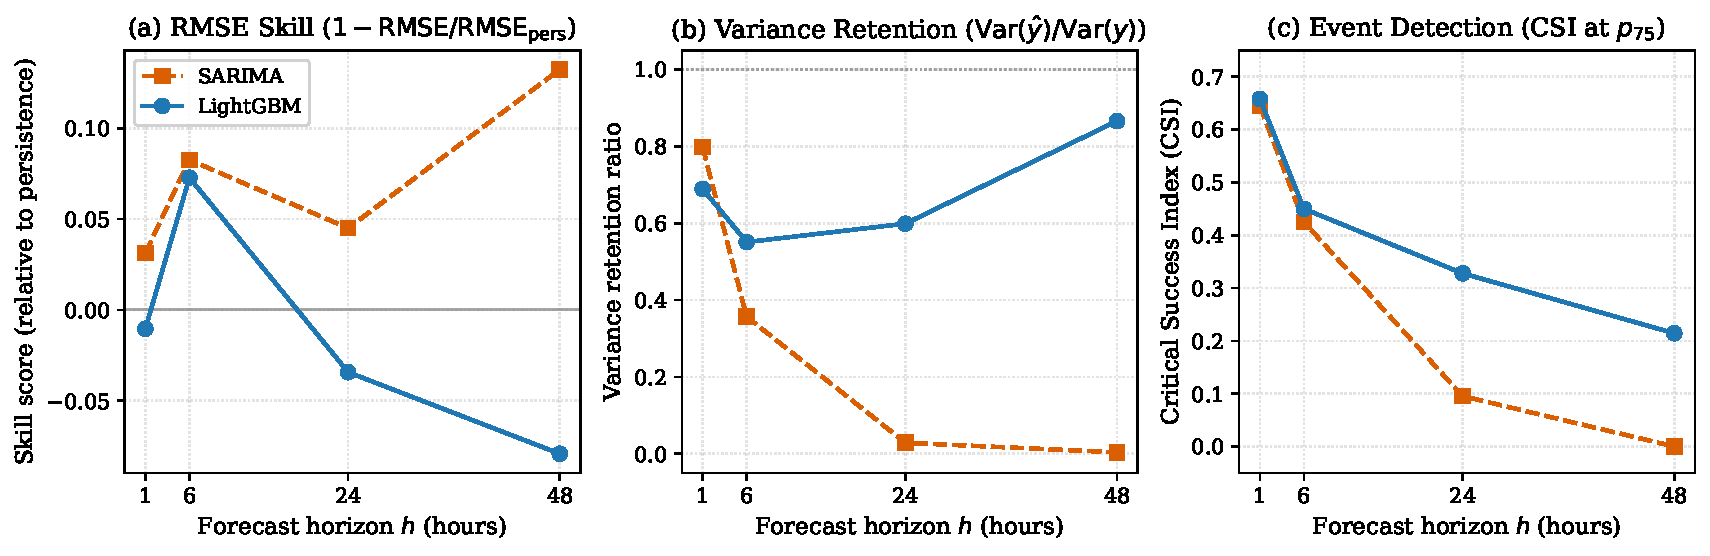
\includegraphics[width=\linewidth]{figures/fig1_horizon_evaluation_divergence.pdf}
\caption{Horizon-wise evaluation divergence between LightGBM and SARIMA across (a) persistence-relative RMSE skill, (b) variance retention, and (c) Critical Success Index (CSI) at the train-derived $p_{75}$ threshold. At $h=48$~h, RMSE skill favors SARIMA ($+0.1325$ vs $-0.0793$), while dynamic fidelity and threshold-event detection favor LightGBM ($\mathrm{CSI} = 0.2144$ vs $0.0000$). Source: \texttt{fig1\_horizon\_evaluation\_divergence.csv}, derived from publication source tables \texttt{pub\_table\_1\_error\_metrics.csv}, \texttt{pub\_table\_2\_dynamic\_fidelity.csv}, and \texttt{pub\_table\_3\_event\_metrics.csv}.}
\label{fig:horizon_divergence}
\end{figure}

\subsection{Multi-Fold Stability and Bounded Ghost-Skill Diagnosis}
\label{sec:results_fold_stability}

Multi-fold analysis confirms that dynamic collapse and complete event failure in 48-h SARIMA forecasts are persistent features across the five expanding evaluation folds (Table~\ref{tab:ghost_skill_structure} and Figure~\ref{fig:fold_stability}).

Across all $5/5$ folds, 48-h SARIMA exhibits dynamic collapse (fold-wise variance retention median $= 0.0007$ [$0.07\%$], range $[0.0005,\, 0.0012]$, maximum fold value $= 0.12\%$) and complete event failure ($\mathrm{POD} = 0.0000$ and $\mathrm{CSI} = 0.0000$ in all 5 folds). Positive continuous error skill ($\mathrm{Skill}_\mathrm{RMSE} > 0$) is present in $3/5$ folds (median $= +0.1124$, range $= [-0.3059,\, +0.2129]$).

The variance-collapse and event-failure components recur in all five folds, whereas the complete three-criterion diagnostic pattern occurs in three of five folds. In this rolling-origin evaluation, the 48-h SARIMA forecasts satisfy the diagnostic definition of ghost skill.

\begin{figure}[ht]
\centering
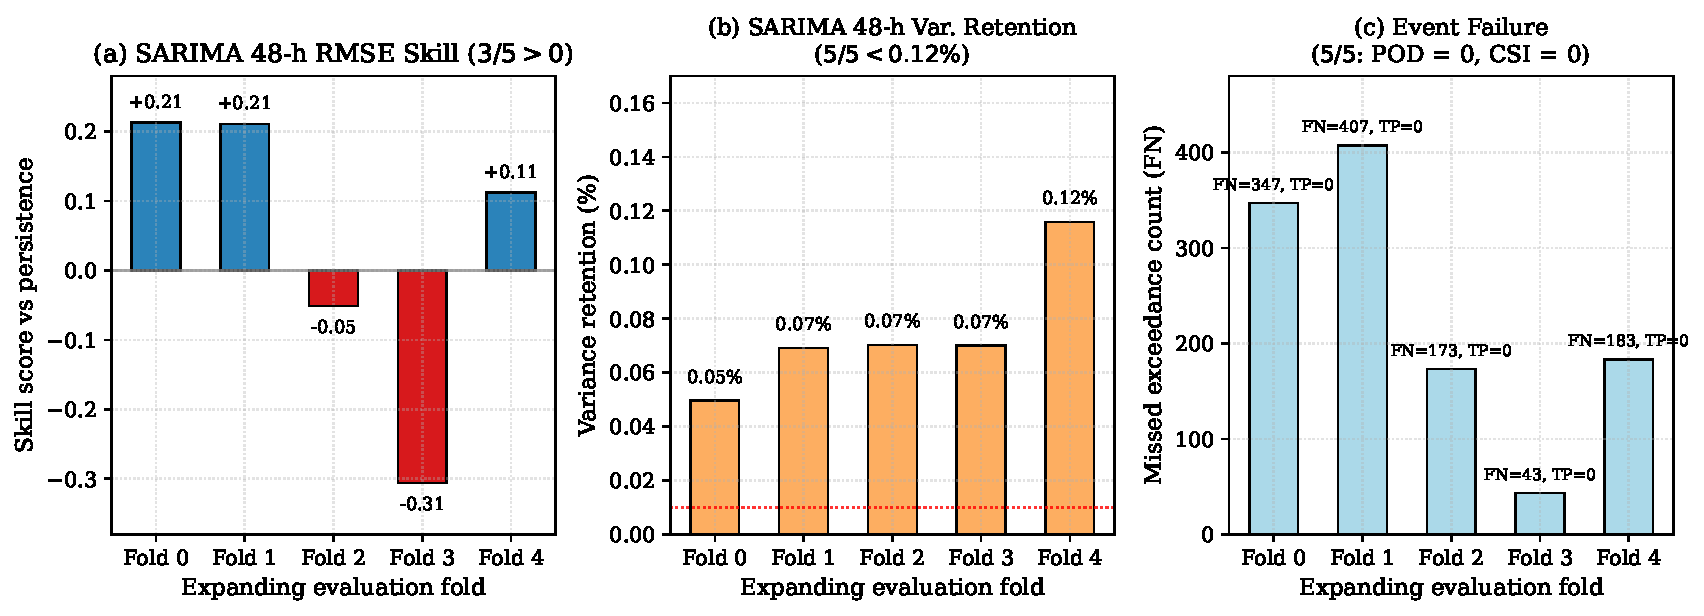
\includegraphics[width=\linewidth]{figures/fig2_sarima48_fold_stability.pdf}
\caption{Fold-wise evaluation of 48-h SARIMA forecasts across five expanding folds: (a) RMSE skill relative to persistence ($3/5 > 0$, median $+0.1124$), (b) variance retention ($5/5 \leq 0.12\%$, median $0.07\%$), and (c) missed exceedances at the train-derived $p_{75}$ threshold ($5/5$: $\mathrm{POD} = 0.0000$, $\mathrm{CSI} = 0.0000$, $\mathrm{TP} = 0$). The variance-collapse and event-failure components recur in all five folds, whereas the complete three-criterion diagnostic pattern occurs in three of five folds. Source: \texttt{fig2\_sarima48\_fold\_stability.csv}, derived from \texttt{fold\_stability\_by\_model\_horizon\_fold.csv}.}
\label{fig:fold_stability}
\end{figure}

% ============================================================
\section{Discussion}
\label{sec:discussion}
% ============================================================

\subsection{Divergence Between Error Skill and Dynamic Fidelity}
\label{sec:disc_main}

\paragraph{Empirical result.}
The central empirical observation of this study is that positive baseline-relative RMSE skill does not imply preserved dynamic fidelity or event representation, leading to an explicit pairwise model-preference reversal. In the evaluated series, 48-h SARIMA achieves superior RMSE skill relative to persistence ($+0.1325$ vs $-0.0793$ for LightGBM), yet simultaneously exhibits near-total variance collapse (variance retention $= 0.0037$), attenuated step-to-step temporal variability ($0.0223$), and detects zero threshold exceedance events ($0/1,153$). LightGBM, despite its inferior RMSE skill, detects 372 exceedance events ($\mathrm{CSI} = 0.2144$), inverting the model preference between continuous error and event criteria.

\paragraph{Diagnostic assessment.}
The joint presence of positive error skill, severe dynamic attenuation, and altered model preference satisfies the operational definition of \emph{ghost skill}. Multi-fold evaluation confirms that the variance-collapse and event-failure components recur across all five expanding folds, whereas the complete three-criterion diagnostic pattern replicates in three of five folds (due to negative continuous skill in Folds 2 and 3). At 24~h, a similar tendency is visible (variance retention $= 0.0286$, $\mathrm{POD} = 0.0992$), reflecting progressive dynamic attenuation across lead times.

\paragraph{Statistical interpretation.}
When an environmental time series exhibits rapid autocorrelation decay, a model that converges toward a near-constant forecast can reduce mean squared error relative to a persistence baseline that continues to track high-variance but lagged observations. However, because this error reduction is achieved through dynamic collapse rather than accurate episode prediction, model selection governed solely by aggregate RMSE skill favors a forecast that is incapable of identifying threshold-defined pollution events.

\subsection{Contextualization: Shrinkage and Variance Attenuation in Forecast Verification}
\label{sec:disc_shrinkage}

The phenomenon of forecast variance attenuation under squared-error loss is mathematically well established \citep{murphy1988,gneiting2011,taylor2001}. For any stationary process under squared-error loss, the optimal point forecast is the conditional mean $\hat{y}_{t+h|t} = \mathbb{E}[y_{t+h}|\mathcal{F}_t]$, which naturally satisfies $\operatorname{Var}(\hat{y}_{t+h|t}) \le \operatorname{Var}(y_{t+h})$. As the forecast horizon $h$ increases and autocorrelation decays ($\rho_h \to 0$), the conditional mean converges toward the unconditional mean $\mu$, driving forecast variance to zero. 

Because the persistence baseline has expected squared error $\mathbb{E}[(y_{t+h} - y_t)^2] = 2\sigma^2(1 - \rho_h) \to 2\sigma^2$, a constant mean forecast $\hat{y} = \mu$ with $\operatorname{Var}(\hat{y}) = 0$ achieves an asymptotic persistence-relative skill of $1 - \sqrt{\sigma^2 / (2\sigma^2)} = 1 - 1/\sqrt{2} \approx +0.293$. 

The contribution of this paper is not claiming to discover this mathematical property, but demonstrating its practical evaluative consequence in environmental forecasting: under identical out-of-sample predictions with common support, standard baseline-relative RMSE skill scores reward this attenuation, selecting a forecast with complete event failure over an alternative model that actively represents environmental dynamics and threshold exceedances. The term \emph{ghost skill} is used strictly as a diagnostic label for this consequential joint pattern, not as a synonym for variance attenuation itself.

\subsection{Interpretive Boundaries}
\label{sec:disc_boundaries}

Several interpretive boundaries apply to the present findings:

\emph{Single-series scope and metadata provenance.}
The evidence derives from a single hourly $\mathrm{PM}_{10}$ series evaluated under a rolling-origin protocol. No station-aggregated, network-wide, or multi-series claim is supported by this evidence. Whether model-preference reversal occurs in other monitoring series, geographic regions, or pollutant contexts is an open empirical question. The evidence is assessed at Grade B provenance pending complete station metadata.

\emph{No causal claim.}
The study documents the empirical coexistence of positive RMSE skill and collapsed dynamic fidelity under the evaluated protocol. It does not isolate model-internal algorithmic mechanisms or establish causal links between specific loss functions and variance decay.

\emph{No universal model claim.}
The finding that 48-h SARIMA exhibits ghost skill in this series does not imply that SARIMA generally produces ghost skill, nor that LightGBM is universally superior across all evaluation criteria.

\subsection{Implications for Environmental Forecast Evaluation Practice}
\label{sec:disc_implications}

The present results suggest that verification of environmental forecasts---and point forecasts in related atmospheric contexts---is more informative when error-based skill is examined alongside dynamic-fidelity and event-based diagnostics \citep{gneiting2011,jolliffe2012,bonas2025}. Evaluating models solely by aggregate RMSE can conceal structural dynamic failure and lead to erroneous model rankings.

Reporting variance retention ($\alpha$), temporal variability ($\tau$), and exceedance metrics ($\mathrm{CSI}$, $\mathrm{POD}$) alongside standard skill scores requires minimal computational overhead and makes potential evaluative divergences transparent. In environmental decision-making, where threshold exceedances and dynamic swings are directly relevant to alert protocols, multi-criteria verification provides an essential safeguard against selecting dynamically collapsed forecasts.

% ============================================================
\section{Limitations}
\label{sec:limitations}
% ============================================================

This study is intentionally bounded in scope:

\begin{itemize}
  \item \textbf{Empirical scope}: The evidence covers a single hourly $\mathrm{PM}_{10}$ series; transferability to other pollutants, temporal granularities, or monitoring networks is not evaluated.
  \item \textbf{Model contrasts}: The evaluation is restricted to a pairwise contrast between two model paradigms (LightGBM and SARIMA) against persistence; it is not a comprehensive model tournament.
  \item \textbf{Feature space}: The lags-only autoregressive design excludes meteorological covariates to isolate the autoregressive dynamic; models incorporating meteorological features may exhibit different fidelity profiles.
  \item \textbf{Diagnostic conventions}: Exceedance events are defined using a train-derived 75th percentile ($p_{75}$) per fold; this is a diagnostic convention, not a statutory air-quality standard.
  \item \textbf{Fold replication}: The complete three-criterion diagnostic pattern replicates in 3 of 5 expanding folds, reflecting fold-level variability in persistence skill.
  \item \textbf{Complementary role}: Dynamic-fidelity metrics are proposed as diagnostic complements to, rather than replacements for, standard error-based verification.
\end{itemize}

% ============================================================
\section{Conclusion}
\label{sec:conclusion}
% ============================================================

Model selection based exclusively on persistence-relative RMSE skill in multi-horizon environmental forecasting can favor a forecast that achieves error reduction while failing to capture dynamic variability or threshold exceedance events. In an audited hourly $\mathrm{PM}_{10}$ series evaluated under rolling origin, 48-h SARIMA forecasts achieve positive RMSE skill relative to persistence ($+0.1325$), yet retain only $0.37\%$ of observed variance and detect none of the 1,153 observed $p_{75}$ events ($\mathrm{POD} = 0.0000$, $\mathrm{CSI} = 0.0000$) across five expanding folds. In contrast, LightGBM yields negative RMSE skill ($-0.0793$) but preserves dynamic variability and detects 372 events ($\mathrm{CSI} = 0.2144$), resulting in an explicit pairwise model-preference reversal.

These results illustrate that positive error-based skill does not guarantee preserved dynamic fidelity or event representation. For environmental forecasting applications where episodic extremes and temporal variability matter alongside average error, evaluating forecasts across continuous error, dynamic fidelity, and threshold event representation provides a necessary diagnostic framework for distinguishing genuine predictive capability from deceptive variance attenuation.

% ============================================================
\section*{Data and Code Availability}
\label{sec:data_availability}
% ============================================================

The analysis code, evaluation scripts, and frozen publication source tables that underpin all numerical results in this manuscript are openly available at \url{https://github.com/fedeg-umh-es/varret-pm10-paper}. The frozen experimental state corresponds to repository commit \texttt{95c9cbdc8c582f5657523c404afa58e61f5e1137}; publication table packaging corresponds to commit \texttt{f233a20ae7eb7411e84eaaa326c3aff87601f628}. The canonical input prediction file (\texttt{predictions\_rolling\_origin.parquet}, SHA-256: \texttt{e7073712ba1a}\allowbreak\texttt{b9f3de29621dfa9c96eec634b86ad7bf66ae37a9c098d15b58c4}) and all derived publication source tables are archived in the repository and can be used to reproduce every number reported in this manuscript \citep{sandve2013}.

% ============================================================
\section*{CRediT Author Contributions}
% ============================================================

Federico Garc\'ia Crespi: Conceptualisation, Data curation, Formal analysis, Investigation, Methodology, Software, Validation, Visualisation, Writing -- original draft, Writing -- review \& editing.
Julio Alberto Ramos Mart\'inez: Conceptualisation, Supervision, Writing -- review \& editing.

% ============================================================
\section*{Declaration of Competing Interests}
% ============================================================

The authors declare that they have no known competing financial interests or personal relationships that could have appeared to influence the work reported in this paper.

% ============================================================
\section*{Acknowledgements}
% ============================================================

The authors used a generative AI assistant for language editing and for \LaTeX{} and reference formatting. All data processing, analysis, results, and scientific conclusions are the authors' own and were verified by the authors, who take full responsibility for the content of this paper.

% TODO AUTHOR: Insert funding statement (grant number(s) and funding body) before submission.

% ============================================================
% BIBLIOGRAPHY
% ============================================================

\bibliography{references}

% ============================================================
% TABLES (SEPARATE PAGES AFTER REFERENCES PER ENVIRONMETRICS GUIDELINES)
% ============================================================

\clearpage
\begin{table}[p]
\centering
\caption{Continuous error metrics by model and horizon.
$\mathrm{Skill}_\mathrm{RMSE} = 1 - \mathrm{RMSE}_\mathrm{model} /
\mathrm{RMSE}_\mathrm{persistence}$; positive values indicate
improvement over causal persistence.
Source: \texttt{pub\_table\_1\_error\_metrics.csv}, experimental commit
\texttt{95c9cbd}.}
\label{tab:error_metrics}
\begin{tabular}{llSSS}
\toprule
Model & Horizon (h) &
  {RMSE ($\mu$g\,m$^{-3}$)} &
  {Persistence RMSE ($\mu$g\,m$^{-3}$)} &
  {$\mathrm{Skill}_\mathrm{RMSE}$} \\
\midrule
LightGBM & 1  & 5.667 & 5.609 & -0.0104 \\
LightGBM & 6  & 9.147 & 9.865 & +0.0729 \\
LightGBM & 24 & 12.802 & 12.377 & -0.0343 \\
LightGBM & 48 & 15.228 & 14.110 & -0.0793 \\
\addlinespace
SARIMA   & 1  & 5.433 & 5.609 & +0.0314 \\
SARIMA   & 6  & 9.050 & 9.865 & +0.0827 \\
SARIMA   & 24 & 11.819 & 12.377 & +0.0450 \\
SARIMA   & 48 & 12.241 & 14.110 & +0.1325 \\
\bottomrule
\end{tabular}
\end{table}

\clearpage
\begin{table}[p]
\centering
\caption{Dynamic-fidelity metrics by model and horizon.
Variance retention $= \operatorname{Var}(\hat{y}) / \operatorname{Var}(y)$;
temporal variability $= \overline{|\Delta\hat{y}|} / \overline{|\Delta y|}$;
amplitude ratio $= \mathrm{IQR}_{95\text{--}5}(\hat{y}) / \mathrm{IQR}_{95\text{--}5}(y)$;
event amplitude retention $= \overline{\hat{y}[y>p_{75}]} / \overline{y[y>p_{75}]}$.
Source: \texttt{pub\_table\_2\_dynamic\_fidelity.csv}, experimental commit
\texttt{95c9cbd}.}
\label{tab:dynamic_fidelity}
\begin{tabular}{llSSSS}
\toprule
Model & Horizon (h) &
  {\begin{tabular}[c]{@{}c@{}}Var.\\retention\end{tabular}} &
  {\begin{tabular}[c]{@{}c@{}}Temp.\\variability\end{tabular}} &
  {\begin{tabular}[c]{@{}c@{}}Amplitude\\ratio\end{tabular}} &
  {\begin{tabular}[c]{@{}c@{}}Event amp.\\retention\end{tabular}} \\
\midrule
LightGBM & 1  & 0.689 & 0.696 & 0.824 & 0.859 \\
LightGBM & 6  & 0.551 & 0.456 & 0.711 & 0.773 \\
LightGBM & 24 & 0.599 & 0.495 & 0.791 & 0.720 \\
LightGBM & 48 & 0.866 & 0.386 & 1.160 & 0.666 \\
\addlinespace
SARIMA   & 1  & 0.798 & 0.764 & 0.899 & 0.898 \\
SARIMA   & 6  & 0.357 & 0.503 & 0.598 & 0.714 \\
SARIMA   & 24 & 0.029 & 0.153 & 0.173 & 0.544 \\
SARIMA   & 48 & 0.004 & 0.022 & 0.063 & 0.507 \\
\bottomrule
\end{tabular}
\end{table}

\clearpage
\begin{table}[p]
\centering
\caption{Exceedance event metrics by model and horizon.
Threshold: training-partition 75th percentile (computed per fold).
POD: Probability of Detection ($\mathrm{TP}/(\mathrm{TP}+\mathrm{FN})$);
CSI: Critical Success Index ($\mathrm{TP}/(\mathrm{TP}+\mathrm{FP}+\mathrm{FN})$);
Event bias: $(\mathrm{TP}+\mathrm{FP})/(\mathrm{TP}+\mathrm{FN})$.
Source: \texttt{pub\_table\_3\_event\_metrics.csv}, experimental commit
\texttt{95c9cbd}.}
\label{tab:event_metrics}
\begin{tabular}{llSSSSSS}
\toprule
Model & Horizon & TP & FP & FN & TN & {POD} & {CSI} \\
\midrule
LightGBM & 1  &  966 &  220 &  283 & 2712 & 0.773 & 0.658 \\
LightGBM & 6  &  727 &  374 &  515 & 2545 & 0.585 & 0.450 \\
LightGBM & 24 &  571 &  532 &  639 & 2329 & 0.472 & 0.328 \\
LightGBM & 48 &  372 &  582 &  781 & 2217 & 0.323 & 0.214 \\
\addlinespace
SARIMA   & 1  &  981 &  272 &  268 & 2660 & 0.785 & 0.645 \\
SARIMA   & 6  &  663 &  319 &  579 & 2600 & 0.534 & 0.425 \\
SARIMA   & 24 &  120 &   47 & 1090 & 2814 & 0.099 & 0.095 \\
SARIMA   & 48 &    0 &    0 & 1153 & 2799 & 0.000 & 0.000 \\
\bottomrule
\end{tabular}
\end{table}

\clearpage
\begin{table}[p]
\centering
\caption{Ghost-skill structure and fold-stability summary.
$\mathrm{Skill}_\mathrm{RMSE}$ and variance retention are pooled
over matching fold--horizon windows.
Fold-wise variance retention: median [min, max] across 5 folds,
reported only for $h \geq 24$~h where fold heterogeneity is material.
Source: \texttt{pub\_table\_4\_ghost\_skill\_structure.csv} and
\texttt{fold\_stability\_summary\_sarima.csv},
experimental commit \texttt{95c9cbd}.}
\label{tab:ghost_skill_structure}
\small
\begin{tabularx}{\linewidth}{llS[table-format=+1.4]S[table-format=1.4]S[table-format=1.4]S[table-format=1.4]X}
\toprule
Model & $h$ (h) &
  {$\mathrm{Skill}_\mathrm{RMSE}$} &
  {\begin{tabular}[c]{@{}c@{}}Var.\ ret.\\(pooled)\end{tabular}} &
  {POD} &
  {CSI} &
  Ghost-skill status \\
\midrule
LightGBM & 1  & -0.0104 & 0.689 & 0.773 & 0.658 &
  Negative skill \\
LightGBM & 6  & +0.0729 & 0.551 & 0.585 & 0.450 &
  Moderate degradation; events retained \\
LightGBM & 24 & -0.0343 & 0.599 & 0.472 & 0.328 &
  Negative skill \\
LightGBM & 48 & -0.0793 & 0.866 & 0.323 & 0.214 &
  Negative skill \\
\addlinespace
SARIMA   & 1  & +0.0314 & 0.798 & 0.785 & 0.645 &
  No ghost skill \\
SARIMA   & 6  & +0.0827 & 0.357 & 0.534 & 0.425 &
  No ghost skill \\
SARIMA   & 24 & +0.0450 & 0.029 & 0.099 & 0.095 &
  Strong candidate; fold heterogeneity \\
SARIMA   & 48 & +0.1325 & 0.004 & 0.000 & 0.000 &
  \textbf{Ghost skill: 3/5 folds} \\
\bottomrule
\multicolumn{7}{@{}p{\linewidth}@{}}{%
  \emph{Note}: At $h = 48$~h, SARIMA fold-wise variance retention:
  median $0.0007$ [$0.07\%$], range $[0.0005,\, 0.0012]$.
  Dynamic collapse in 5/5 folds; complete event failure in 5/5 folds;
  positive error skill in 3/5 folds; full ghost-skill pattern in 3/5 folds.}\\
\end{tabularx}
\end{table}

\end{document}
